\documentclass[draft,linenumbers]{agujournal}

\draftfalse

\usepackage{hyperref}
\hypersetup{
colorlinks=true,
linkcolor=blue,
filecolor=magenta,
urlcolor=cyan}

\journalname{Journal of Advances in Modeling Earth Systems (JAMES)}

\begin{document}
%tentative author list...
\authors{Rosie A. Fisher\affil{1,1},
William R. Wieder\affil{1,3},
Benjamin M. Sanderson\affil{3},
Charles D. Koven\affil{4},
Keith W. Oleson\affil{1},
Chonggang Xu\affil{5},
Joshua Fisher\affil{6},
Mingjie Shi\affil{6},
Anthony P. Walker\affil{7},
David M. Lawrence\affil{1}
}

\title{Parametric controls on vegetation responses to biogeochemical forcing in the CLM5}
\author{Rosie Fisher}
\date{June 2019}

\affiliation{1}{National Center for Atmospheric Research, Table Mesa Drive, Boulder, Colorado, USA}

\affiliation{2}{Centre Europ\'een Research et de Formation Avenc\'ee en Calcul Scientifique, Toulouse, France}

\affiliation{3}{Institute of Arctic and Alpine Research, University of Colorado, Boulder Colorado, USA}

\affiliation{4}{Lawrence Berkeley National Laboratory, Berkeley, California, USA}

\affiliation{5}{Los Alamos National Laboratory, Los Alamos, New Mexico, USA}

\affiliation{6}{Jet Propulsion Laboratory, California Institute of Technology, Pasadena, California, USA}

\affiliation{7}{Oak Ridge National Laboratory, Oak Ridge, Tennessee, USA}

\correspondingauthor{Rosie Fisher}{rfisher@ucar.edu}


\begin{keypoints}
\item The Community Land Model, version 5, contains numerous modifications to representations of the vegetation carbon and nitrogen cycles.\\

\item The control model state, and it's responses to CO$_{2}$ and nitrogen addition. are sensitive to parameter choice, and parameter responses further vary with pre-fertilization water and nitrogen limitation. \\

\item Parameters controlling nitrogen fixation rates dominate fertilization responses. Many other fertilization responses are modified indirectly, via changes in the pre-fertilization state. 
\end{keypoints}

\begin{abstract}
Future projections of land carbon uptake in Earth System Models are affected by land surface model responses to both CO$_{2}$ and nitrogen fertilization. The Community Land Model (CLM), version 5, contains a suite of modifications to carbon and nitrogen cycle representation. Globally, the CLM5 has a larger CO$_{2}$ responses and smaller nitrogen response than its predecessors. To improve our understanding of the controls over the fertilization responses of the new model, we assess sensitivity to eight parameters pertinent to the cycling of carbon and nitrogen by vegetation, both under present-day conditions and with CO$_{2}$ and nitrogen fertilization.

 The impact of fertilization varies with both model parameters and with the balance of limiting factors (water, temperature, nutrients, light) in the pre-fertilization model state.  The model parameters that impact the pre-fertilization state are in general not the same as those that control fertilization responses, meaning that goodness of fit to present-day conditions does not necessarily imply a constraint on future transient projections. Where pre-fertilization state has low leaf area, fertilization-induced increases in leaf production amplify the model response to the initial fertilization via further increases in photosynthesis.  Model responses to CO$_{2}$ and N fertilization are strongly impacted by how much plant communities can increase their rates of nitrogen fixation, and also directly affected by costs of N extraction from soil and stoichiometric flexibility. Illustration of how parameteric flexibility impacts model outputs should help inform the interpretation of carbon-climate feedbacks estimated by in fully-coupled Earth system model simulations. 
\end{abstract}

\section{Introduction}
The response of the terrestrial biosphere to carbon dioxide enrichment and increasing nitrogen (N) deposition represents a major source of uncertainty in predictions of the evolution of the climate system (\cite{friedlingstein2006},  \cite{arora2013}, \cite{friedlingstein2014}). In the CMIP5 multi-model inter-comparison, the smallest response to CO$_{2}$ forcing was predicted by the Community Land Model v4 (CLM4, \cite{thornton2007}, \cite{lawrence2011}), the only model in that comparison that represented the impacts of nitrogen availability on plant growth, leading to suggesting that the addition of nitrogen limitation might substantially reduce the capacity for vegetation to respond to CO$_{2}$ fertilization (and hence reduce the degree to which the terrestrial biosphere can mitigate increasing atmospheric CO$_{2}$. 

The newly-released CLM version 5  (CLM5, \cite{lawrence2018}) includes numerous updates relative to the CLM4 and CLM4.5  (\cite{oleson2013} ). The introduction of several new dynamical features, including substantial modification of the vegetation nitrogen cycling, a new plant hydrodynamics scheme (\cite{kennedy2019}), altered surface hydrology, snow physics and dynamic crop representation, has implications for responses to environmental forcing. \cite{wieder2019} report the global carbon cycle implications of these changes and note that, in CLM5, carbon uptake responds more strongly to CO$_{2}$ and less strongly to N fertilization than its predecessors, with both fertilization responses being closer to experimental results than the previous versions of the model. 

Large quantities of analysis and computing resources will likely be devoted to assessing the impacts of transient CO$_{2}$ and N on CMIP class models, such as CLM5, in the context of global biogeochemical feedback analysis (e.g. \cite{arora2013}, \cite{friedlingstein2014}). Land surface models, in particular the elements related to biogeochemical cycling, are nonetheless subject to very high degrees of parametric and structural uncertainty (\cite{bonan2018}, \cite{zaehle2014}) Given this,  we consider that the illustration of how parametric choices affect the responses to biogeochemical forcing in such models is an important feature of model documentation.

In this paper, to that end, we describe the new components of the biogeochemical cycling in CLM5, and assess the sensitivity of the CLM5 model parameterization of ecosystem biogeochemistry. We use a range of single site simulations, combined with one-at-a-time parameter uncertainty analyses, and CO$_{2}$ and N fertilization experiments, to investigate the dynamics of the model under steady-state and step-change modifications in forcing. We further highlight areas of process and parametric uncertainty that appear to require greater attention in future model development and testing cycles.

The majority of land surface model sensitivity tests, uncertainty quantification efforts and calibration exercises are conducted under present-day conditions (\cite{fer2018}, \cite{lu2018}, \cite{dietze2014}, \cite{ricciuto2018}). Predicted global biogeochemical feedbacks, however, are in principle related to the response of the system to forcing, and not necessarily to those system properties that control the mean state.  Thus, our motivating questions here are:

1. Are parameters that dominate responses to CO$_{2}$ and nitrogen fertilization also dominant over the pre-fertilization model state?

2. How do fertilization impacts and parameter sensitivities vary with site conditions, as expressed via water and nutrient limitations. 

The analysis herein does not focus on the relative fit of the model to the data collected at the individual sites. The fit at individual sites of the globally adjusted model typically cannot be seen as indicative or otherwise of its skill in the absence of specific parameterization using the local vegetation, soil and hydrological characteristics. A focus on model fit at individual sites would preclude detailed consideration of how parameter variation impacts fertilization responses, as presented here. Assessment of the skill of the CLM5 model against a broad suite of globally-relevant data products and manipulation experiments is the focus of \cite{lawrence2018} and \cite{wieder2019}. Future studies will consider the impact of alternative parameterizations, informed by these analyses, on the global performance and skill of CLM5.

\section{Methods}

\subsection{CLM5}
 Version 5 of the CLM was released to the research community in 2018 as part of the CESM2.0 release, and open-source releases and development are housed at \url{https://github.com/ESCOMP/ctsm/}. An overview of model developments is presented within this special issue by \cite{lawrence2018}, a description of the global nitrogen cycling by \cite{wieder2019}/. The plant hydraulics model is documented by \cite{kennedy2019}. Further manuscripts will describe the crop, urban and land use models, sensitivity to forcing and calibration of fast-timescale processes.
 
\subsection{Updates to biogeochemistry Cycling in the CLM5}
The CLM5 biogeochemistry scheme builds on the initial implementation of carbon-nitrogen interactions in CLM4 (\cite{thornton2007}),  and on modifications to the biogeochemical cycling (notably, a vertically stratified soil decomposition processes, and a slowing of the soil mineral N loss pathways) included in the CLM4.5 (\cite{koven2013}, \cite{bonan2012}). 

 A full technical description of the CLM5 is beyond the scope of this paper and is available as an appendix to \cite{lawrence2018} and also online at \url{(https://escomp.github.io/ctsm-docs/doc/build/html/tech_note/index.html)}.

In this paper, we focus on the response to CO$_{2}$ and nitrogen deposition, which are primarily mediated by the biogeochemical processes within the model. The primary changes to the biogeochemical cycling in CLM5 are within the vegetation nitrogen cycle, wherein the model contains three new prognostic elements that are likely to impact responses to fertilization.

Firstly, the  `LUNA' module (Leaf Utilization of Nitrogen for Assimilation),  simulates distribution of N between different leaf assimilation processes (\cite{xu2012}, \cite{ali2016}). Most land surface models predict photosynthetic parameters directly from leaf nitrogen content (\cite{kattge2009}, \cite{bonan2012}). This method, however, appears to be a poor means of capturing variation in photosynthetic capacity in time and space and responses to climatic change (\cite{walker2017}). There is significant evidence that plant photosynthetic capacity can respond to environmental conditions, including CO$_{2}$ fertilization (\cite{ainsworth2007}), changing temperature (\cite{hikosaka2005}), irradiance (\cite{niinemets1998}) and soil moisture (\cite{keenan2009}).  LUNA predicts the optimal partitioning of N among the maximum rate of carboxylation $V_{c,max}$, the maximum rate of electron transport $J_{max}$, and other leaf N components for a given leaf nitrogen (per unit area) and environmental boundary conditions (CO$_{2}$, temperature, humidity, soil moisture, radiation and day length), assuming co-limitation of photosynthesis by both electron capture and carboxylation processes.  $V_{c,max}$ is thus primarily controlled by the N per unit leaf area $N_{area}$ and the prevailing meteorology. The capacity of the LUNA model to represent appropriate responses to temperature and CO$_{2}$ was demonstrated by \cite{xu2012} while the global calibration and the geographical predictions of the model were described by \cite{ali2016}.

Secondly, the `FUN' (Fixation and Uptake of Nitrogen) model was incorporated into CLM5. FUN simulates the dynamics and carbon economics of N acquisition from the environment, building on (\cite{fisher2010fun} and \cite{brzostek2014} and \cite{shi2016}). A major issue confronting N cycle models is how to manage 'excess' carbon under conditions where carbon assimilation is faster than that which can be supported by nutrient uptake (\cite{dekauwe2014}). Previous versions of CLM model reduced the gross photosynthetic flux down to the level at which growth could be supported by N uptake. This process occurred after the calculation of stomatal conductance (which is linked to assimilation rates via the Ball-Berry model) and therefore created inconsistencies between C assimilation and water cycling, especially under conditions of N limitation, as discussed extensively in the literature (\cite{medlyn2011}, \cite{bonan2012}, \cite{dekauwe2014}, \cite{walker2014}). The FUN model, in contrast, employs the principle that for the alternative sources of nitrogen acquisition by plants (active uptake from soil, retranslocation from senescent tissues, and symbiotic N fixation) there is a concurrent cost in terms of carbon (\cite{bloom1985}, \cite{jiang2017}, \cite{terrer2018}) which is determined by the abundance of nitrogen in the soils and plant tissues and the temperature-dependant cost of N fixation. Within FUN, plants spend excess carbon for nitrogen uptake preferentially using pathways which are `cheaper' to them. Where N is scarce in the environment, carbon that would otherwise have been used for plant growth can be deployed to acquire (pay for) more N. Thus, N limitation leads to both reduced growth and higher expenditure of C on N uptake.   The switching of N uptake to cheaper pathways results in the preferential use of symbiotic N fixation when soil mineral N concentrations are low (\cite{vitousek2002}), whereas CLM4 and CLM4.5 predicted N fixation as a linear function of net primary productivity (\cite{cleveland1999}; \cite{wieder2015}).   The FUN model is documented within the CLM technical note at \url{https://escomp.github.io/ctsm-docs/doc/build/html/tech_note/FUN/CLM50_Tech_Note_FUN.html}. 
 
Thirdly, CLM5 contains the capacity to modify tissue C:N ratios with spatial and temporal variation in the cost of N uptake.  Plant trait databases (e.g. \cite{kattge2011}) typically indicate a wide variability in tissue N concentrations within a single plant functional type (\cite{wright2005}). \cite{ghimire2016} introduced the capacity for variable tissue C:N ratios, whereby the total nitrogen supply in each timestep is partitioned between tissues in proportion to their relative 'demand' terms (ascertained from the target C:N ratio and the carbon allocated to the pool).  The FUN model used in CLM5 was originally conceived in the context of a static tissue C:N ratio. Carbon is allocated between growth and N uptake in a manner that exactly tracks the target C:N ratio. To allow a variable C:N ratio in the context of FUN, it is necessary to modify how much C is expended on N uptake vs on growth from this default calculation. The degree to which tissue C:N content varies as N becomes limiting is unclear in the literature, and N cycle models typically include semi-heuristic and/or bounded representations of tissue N adjustments under N limited conditions (\cite{zaehle2010},\cite{ghimire2016}). Here we include a placeholder algorithm that modifies C:N ratios with 1) the environmental cost of N acquisition and 2) the degree to which the plant is already far from its target N content. When N is scarce in the environment, less C is spent on uptake, increasing C:N ratios. When plants become N limited and C:N ratios increase, however, expenditure increases. This algorithm is also documented in the CLM5 technical description ((\url{(https://escomp.github.io/ctsm-docs/doc/build/html/tech_note/index.html)}) and includes three tuning parameters ($flexcn_{a}$, $flexcn_{b}$ \& $flexcn_{c}$) the sensitivity of which is investigated here.

\subsection{Sites}
We utilized four observational flux tower sites, in order to capture a range of environmental conditions, across tropical evergreen broadleaf forest (Caxiuan\~a, -1.9$^{o}$N, -51.4$^{o}$E),  sub-alpine evergreen forest (Niwot Ridge, 40.3$^{o}$N, -105.4$^{o}$E), temperate deciduous broadleaf forest (Harvard Forest, 42.5$^{o}$N -72.2$^{o}$E) and seasonally dry evergreen needleleaf forest (Metolius Forest, 44.5$^{o}$N -121.6$^{o}$E).  Each site was driven with the available site-specific meteorological data. Soil texture, color, depth and, plant functional type composition were taken from previous model validation exercises undertaken at these sites \cite{bonan2012} for Metolius and Harvard Forest, \cite{fisher2007} for Caxiuan\~a and \cite{bonan2013} for Niwot Ridge.   We note here that our use of a small number of single sites cannot fully describe the environmental conditions under which the model is applied. Instead, our aim is to provide detailed illustrations of how model parameter choices impact a model outputs under a range of realistic forcing conditions. Conducting and analysing these simulations globally is beyond the scope of this study, but investigations of the response of global biogeochemical feedback strength to the important dimensions of parameter space identified by this investigation will provide the basis of future studies. 

\subsection{Simulation Protocol}
We spun up the default version of the model for 400 years at each site, in 'accelerated spin-up' mode (whereby the decomposition of slower cycling carbon and nitrogen pools is increased for the duration of the spin-up, and the pool sizes are modified accordingly at the end of the spin-up - see (\cite{lawrence2018}). We used pre-industrial CO$_{2}$ concentrations (274ppm) and recycled the available site-level half-hourly meteorological inputs for the duration of the simulations. 400 years was sufficient to bring all soil and vegetation carbon and nitrogen pools into equilibrium. Subsequent to this, parameters were perturbed (see below), and a second spin-up conducted for 180 years for each site, parameter and value combination, with accelerated mode turned off. Restarting from the state at the end of the perturbed parameter spin-ups, we ran 'control' transient simulations for each site and parameter combination starting in 1760 and invoking historical transient CO$_{2}$ and N deposition until 2018.

For each site/parameter/value combination, we also ran one elevated CO$_{2}$ and one elevated nitrogen deposition simulation. Following \cite{wieder2019}, who conducted global runs with the default parameterization of the model, we increased CO$_{2}$ to 550ppm, starting in 1998 and for Nitrogen, we added 5gN $m^{-2}$/year, also starting in 1998. 

\subsection{Perturbed Physics Ensemble (PPE)}
The CLM5 has a large array of parameters that might have direct and indirect impacts on biogeochemical cycling in the model.  Here we focus on an array of thirteen parameters, chosen for their direct mechanistic impacts on responses to CO$_{2}$ and N fertilization. These parameters are narrowed down from the much larger complete set of CLM5 parameters (which will not enumerate here, since calculation of this number in a model as complex as CLM5 is a scientific exercise in its own right) using a process informed primarily by the model structure, as well as the extensive iterative investigations of the CLM5 model during the development process.  We focus here on biogeochemically important inputs. Parameters relevant to the hydrology and surface energy balance processes (with the exception of the stomatal slope) since sensitivity to these will be assessed by studies currently underway, and parameters of the new plant hydraulics scheme are discussed in \cite{kennedy2019}.

To reduce the complexity involved in understanding and attributing changes in model behaviour with parameter variation, we conducted one-at-a-time (OAAT) perturbations of the parameters around the default state, which (compared to a global parameter sensitivity analysis) allows more straightforward visualization and interpretation of the results.  At each site, we conduct simulations with five values of each parameter (one of which is the default) across the ranges described below. We recognize that a global parameter sensitivity analysis would also be of interest, and indeed have conducted many such analyses. We concluded that OAAT analysis provides clearer insight into the functionality of the parameters with respect to biogeochemical forcing. 
\subsection{Default parameter determination}
During the development of CLM5, we conducted extensive testing into the possibility of inverse-calibration of the model using neural network derived emulators, in conjunction with a variety of gridded global data products. We did not use the results of this effort for a variety of reasons, including,  1) the high dimensionality of the space, 2) the degree of non-orthogonal behaviour in the parameter response surfaces, 3) the tendency of the modeled ecosystem to die under lower pre-industrial CO$_{2}$ conditions when calibrated using present-day CO$_{2}$, 4) the dominance of high productivity areas over the calibration of a particular PFT at the expense of marginal areas, and the resulting effect that those marginal areas die off in model spin-up, 5) the subjectivity in weighting of the various observational data products and 6) philosophical issues concerning whether the structural validity of the calibrated model could be independently assessed, given the sparsity of validation datasets. The parameterization used in the default version of the model consequentially utilized the mean trait values where possible from trait datasets (\cite{lawrence2018}) in combination with targeted manual tuning of parameters (including allocation parameters and Nitrogen costs) that were less well constrained by data, to avoid excessively unrealistic values for some model simulated states. We recognize that this more subjective calibration method is less than ideal, and ongoing studies will focus on more limited scope calibration attempts to overcome the difficulties described above, as illustrated by \cite{fer2018}. 

\subsubsection{Parameters selected for perturbation experiment}
The parameters included in our sensitivity analysis are listed in Table \ref{table_ranges}. Their impact on model functionality is described below.  The shorthand version of the parameter name is given in italics.  

\textbf{Specific Leaf Area}, \emph{`SLA'}, is a parameter common to almost all land surface models, which determines the area of leaves (in m$^{2}$) derived from one gram of leaf biomass. High SLA values correspond to thinner, 'cheaper' leaves which lead to thicker vegetation canopies and greater interception of light. In CLM5 high SLA leaves also have lower N per unit area (given a target mass-based C:N ratio) and thus lower photosynthestic capacity per unit area.

\textbf{Fine root mass per unit leaf mass}, \emph{`froot\_leaf'}, is the (constant) ratio of fine root biomass to leaf biomass. In CLM5, fine root biomass affects the capacity of vegetation to acquire both water and nutrients via the resistance of the rhizosphere to water flow, and the cost of N acquisition in the FUN model, respectively. Lower values should in principle incur a cost to vegetation in terms of below-ground resource acquisition.  The carbon allocation in CLM5 uses a fixed-fraction approach, with constant ratios between, leaf, fine roots, stem and coarse root allocation. As such, the carbon allocation scheme is thus capable of generating physiologically sub-optimal leaf area index values, for example, with some of the canopy in negative carbon balance. Newer codes within the CLM framework (e.g. the FATES model, https://github.com/NGEET/fates, \cite{fisher2015}m \cite{fisher2018vegetation}) account for this issue by removing leaves in negative carbon balance. 

 \textbf{Stem to leaf mass ratio}, \emph{`stem\_leaf'}, controls the fraction of biomass to stem tissues as a fraction of the leaf allocation. Increases in this parameter both decrease the leaf area index (LAI, m$^{2} m^{-2}$) achievable for a given amount of (C and N) allocation to growth, and increase the equilibrium woody biomass. Woody biomass in CLM5 has no functionality and thus there is no cost to plants associated with low values of this parameter).

\textbf{Nitrogen costs}, \emph{`n\_costs'}, are a set of parameters that determine the environmental cost of Nitrogen uptake from the soils. The FUN model introduces the concept of carbon payments for active N uptake, using a bulk approach to account for the costs to plants of low environmental N availability, including; carbon expended on root exudates, symbiotic relationships with soil fungi, expenditure on fine root growth and/or increased metabolic rates to support active uptake. Therefore, uncertainties associated with the cost functions, in particular, are large. These six parameters were defined and calibrated by \cite{brzostek2014}. In CLM5, we maintain the ratios of the parameters as defined by the previous FUN model calibration, but allow the magnitudes of the parameters to change concomitantly, since the definitions of soil N availability vary between CLM5 and \cite{brzostek2014}. The six \emph{'n\_costs'} parameters include \emph{ekc\_active} and \emph{ekn\_active}, the rate constants that relate the cost of ectomycorhhizal uptake to the fine root carbon pool (\emph{ekc\_active}) and soil N concentration (\emph{ekn\_active}), respectively and their counterparts \emph{akc\_active} and \emph{akn\_active} for arbuscular mycorrhizal uptake, and \emph{kc\_nonmyc} and \emph{kn\_nonmyc} for non-mycorrhizal active uptake. 

\textbf{The fraction of carbon that can be used for fixation}, \emph{`fracfixers'}, is the fraction of the net primary production (NPP) or gross primary productivity (GPP) minus autotrophic respiration (not including carbon spent on N uptake, $r_{auto}$) that can be used for symbiotic N fixation.  It is thus a proxy for the ecosystem-level fractional productivity of symbiotically N-fixing plants. The constant \emph{`fracfixers'} parameter here acts in lieu of, for example, a prognostic model of N fixer distributions, or an input map of their abundance, both of which could plausibly be added in future generations of CLM. 

\textbf{Leaf carbon:nitrogen target}, \emph{leafcn}. CLM5 uses the concept of a 'target' leaf C:N ratio, around which flexibility is allowed, given the environmental costs of Nitrogen. As with most land surface schemes, higher leaf N concentrations lead to both higher maintenance respiration costs and higher photosynthetic capacity (in this case via the LUNA model).  

\textbf{Slope of the stomatal conductance model}, \emph{medlyn\_slope}. CLM5 replaced the Ball-Berry stomatal conductance scheme with the Medlyn stomatal conductance scheme (\cite{medlyn2011}). The slope parameter determines the degree of stomatal opening for a given combination of assimilation capacity, CO$_{2}$ and vapour pressure deficit, in the absence of plant hydraulics limitations. Thus, is it intrinsically linked to the response of ecosystems to CO$_{2}$. 

\textbf{C:N flexibility }, \emph{cn\_flex\_a, cn\_flex\_b, \& cn\_flex\_c},  as described in the CLM5 technical note, determine the response of tissue C:N ratios to depletion of N in both the environment and the plant tissues themselves. Only the thid parameter (c) had an important impact in this sensitivity analysis, and so we focus here on the impact of that parameter. 

Other variables we tested in earlier versions of this analysis included rate constants controlling the growth and maintenance respiration rates, the fraction of ectomycorrhizal fungi, and parameters 'a' and 'b' of the flexible C:N ratio model. None of these had important impacts on the fertilization responses, and growth and respiration rates affected the model state in a linear and predictable fashion. They are omitted here for the sake of simplification, but data can be accessed via the available simulations. 

\subsubsection{Parameter Ranges}
\emph{SLA} and \emph{leafcn} are readily observable and thus among the most common traits represented in the TRY plant trait database (\url{www.try-db.org}). We derive values from the analysis by (\cite{kattge2011}) for their mean and distribution. For both parameters, values are log-normally distributed. We here take the PFT average log-normalised standard deviation range from TRY and apply it across all PFTs (thus the lower bounds are closer to the mean than the higher bounds, Table \ref{table_ranges}). The range of \emph{fracfixers} and was set to vary from 0 to 100\% of ecosystem productivity being available for fixation.  \emph{medlyn\_slope} varies across the stndard errors reported in \cite{dekauwe2015}. Reasonable ranges of the \emph{cn\_flex} parameters are unknown, since these physiological controls are poorly understood. Thus, we explore an order of magnitude in each direction from the default, to obtain an understanding of the general sensitivity to this parameterization. The same issues apply to $N_{costs}$ parameters. 

\subsubsection{Responses to forcing}
We calculated the impacts of the CO$_{2}$ and N deposition by assessing the ratio of the fertilized to control simulations, averaging years 15-19 after fertilization began. For some parameter values, the constraint on growth placed the control system in a state close to or at death (zero live carbon pools). Addition of N or CO$_{2}$ therefore caused either a very strong recovery of the plants, or no recovery at all where biomass was already zero, leading to some large non-linearities in the relationship between parameters and environmental forcing. To focus on the responses of parameter combinations that give more reasonable initial vegetation conditions, parameter combinations that caused LAI to be less than 60\% of the control simulation value were excluded from the fertilization plots.

\section{Results}
Our analysis used four sites, with eight parameters perturbed to four different values, each of those with control, CO$_{2}$ and N fertilization simulations.  We examine the parametric responses of five output variables chosen for their importance in the overall biogeochemical system (GPP, NPP, LAI, leaf nitrogen per unit area ($N_{leaf}$, gN m$^{-2}$), and total vegetation carbon (g m$^{-2}$). We did not look at soil output variables as our parameter analysis is focused on vegetation responses. 

In this section we assess first the impacts of parametric variation on the system state and second the responses to carbon and nitrogen fertilization. We do not focus on the goodness of fit to observations, because our aim is to discern the primary parametric controls over CO$_{2}$ and N fertilization responses, and including extensive data-fitting and calibration experiments (including on parameters mostly unrelated to C and N cycling) would detract from this goal. 

\subsection{Overall system state}
The parameter responses of the site-level water and nitrogen limitation (see below) in the control (unfertilized) parameter ensemble are shown in figure \ref{btran state}. GPP, NPP, LAI, $N_{leaf}$ and total vegetation carbon are shown for the Niwot Ridge, (Figure \ref{NR1 state}), Caxiuan\~a (Figure \ref{CAX state}), Harvard Forest (Figure \ref{HVF state}) and Metolius (Figure \ref{MET state}) sites. In each of these figures, the y-axis corresponds to the output variable and the x-axis represents the range of parameter perturbation with -1 to +1 corresponding to the range of variation in each parameter, depicted in Table \ref{table_ranges}. Lines of differing colors illustrate responses to variation in the thirteen target parameters, with the central crossover point in each figure corresponding to the default case.

\subsubsection{Water and N limitation across sites}
The four sites varied in the degree to which they are limited by water and N availability in the control state (Figure \ref{btran state}). Water limitation in CLM5 can be expressed via a model property termed $B_{tran}$, which is calculated as a function of the (prognostic) leaf water potential. $B_{tran}$  is used to reduce assimilation and thus stomatal conductance by scaling the photosynthetic capacity, $V_{c,max}$. Leaf water potential and $B_{tran}$ vary diurnally, so we use the average daily minimum ($B_{tran,mn}$) here as a metric of drought stress (1 is no drought stress, 0 is total stomatal closure). For N limitation, the percentage of total NPP (where NPP is GPP-$r_{auto}$) that is used to pay for nitrogen uptake (PNU) is a direct indicator of how N stress affects the carbon budget. 

The Caxiuan\~a site (CAX) experienced substantial drought stress and little nutrient stress ($B_{tran,mn}$ $\sim$0.6, PNU$\sim$13\%). Niwot Ridge (NWR) experienced substantial amounts of drought and N limitation, ($B_{tran,mn}$, $\sim$0.55, PNU$\sim$21\%). Harvard Forest (HVF) site had very little drought stress, and moderate N limitation ($B_{tran,mn}$ $\sim$0.96, PNU$\sim$15\%).  Metolius (MET)  had some drought stress and the least nutrient stress ($B_{tran,mn}$ $\sim$0.86, PNU$\sim$10\%).  

Thus, the sites chosen span a range of initial limiting conditions. Underlying limitations by different boundary conditions (water, nutrients, light, temperature) affect the ability of the system to respond to fertilization and/or parameter modifications, as we describe further in the following sections. 

\subsubsection{Parametric control over system state}
In this section, we discuss the impacts of the parameter variation on the initial model state.  Many parameters have both first-order direct impacts, and then further impacts via other parts of the model. Here we attempt to illustrate how these mechanisms operate in CLM5 within the parameter space explored here. 

At all sites, specific leaf area (\emph{slatop}) has a large first-order impact on LAI, and on $N_{leaf}$ (Figure \ref{NR1 state}), as expected, since it is used directly in the calculation of both of these quantities. The impact of SLA on GPP is always positive, despite the thinner leaves having lower N, and thus lower photosynthetic capacity, per unit area of leaf. The impact of SLA on NPP can, however, sometimes be negative (CAX, NWR), since the fixed-fraction allometry model in CLM5 can generate shaded leaves that are in negative carbon balance at high LAI. 

The root:leaf ratio (\emph{froot\_leaf}) has numerous impacts, including 1) on LAI, via tissue allocation fractions , 2) on NPP, via changes in maintenance costs of fine root pools, 3) on the uptake of water (via root length density) and 4) on nutrient limitation through root-mediated N uptake costs. The first two impacts represent the costs of more roots, and the latter two their benefits. CAX and HVF exhibit higher LAI with fewer roots. NWR has large reduction in LAI (and GPP \& NPP) with fewer roots. MET exhibits a mixed response crossing an optimal value. \emph{froot\_leaf} is a primary control over drought stress at both NWR and MET ( Figure \ref{btran state}) indicating the impact of mechanism '3' here, for very low root densities.

Low values of \emph{stem\_leaf} ratio resulted in higher LAI at all sites, as well as declines in total vegetation carbon. At NWR, the parameter range crosses a local maximum for vegetation carbon, since increases in NPP are non-linear with respect to leaf investment, resulting in lower vegetation biomass overall. At all other sites, the impact of increasing leaf allocation is to invoke large increases in LAI and NPP. Lower stem allocation and higher LAI increase the N demand, reducing $N_{leaf}$ and increase PNU at Niwot Ridge and Metolius in Figure \ref{btran state}). 

Increasing $N_{costs}$ increases the respiration losses associated with nitrogen uptake.  All sites showed a moderate decline in LAI, NPP, GPP and vegetation carbon when costs were high, but lesser impacts when costs were reduced (Figures \ref{NR1 state}, \ref{CAX state} \ref{HVF state}, \ref{MET state}). In contrast to the allocation parameters, $N_{costs}$ does not appear to be a first-order control over the pre-fertilization system state. 

Increasing \emph{fracfixers} affects the maximum amount of carbon that plants can pay towards symbiotic nitrogen uptake (N fixation). For all sites and variables here, it has a relatively moderate and positive impact on the control state. As is the case for $N_{costs}$, \emph{fracfixers} does not appear to be a first-order control over the pre-fertilization system state.

Changing \emph{leafcn} over one standard deviation from the mean TRY values, had substantial impacts on all the output variables at all sites. Higher \emph{leafcn} values decrease $N_{leaf}$, decreasing photosynthetic capacity and GPP.  In particular, at MET and HVF the higher \emph{leafcn} values had $N_{leaf}$ and photosynthetic capacities so low that GPP was almost zero (Figures \ref{HVF state}, \ref{MET state}).  GPP continues to increase almost linearly with declining \emph{leafcn}  (increasing $N_{leaf}$) at all sites except HVF, indicating a lack of saturation of photosynthesis with respect to photosynthetic capacity.  This is consistent with the analysis by \cite{lawrence2018} who find that V${_c,max}$ numbers in CLM5 might be low compared to observations.  For NPP, respiration costs of modified $N_{leaf}$ and altered PNU (Figure \ref{btran state}) buffered the larger changes in GPP. At CAX, for example, the lowest \emph{leafcn} had a GPP 225 gC/m$^{2}$/y higher, while the corresponding NPP increase was only 52 gC/$m^{2}$/y.

Changes in \emph{medlyn\_slope}, the stomatal slope parameter, across the range shown here, have limited impacts on the pre-fertilized system state, with the exception of NWR, where lower values of the slope parameter generated higher photosynthesis, consistent with this site experiencing severe drought stress and thus benefiting from increased water efficiency. 

\emph{cn\_flex\_c} affects the degree to which plants attempt to maintain tissue C:N values near to their target when environmental costs are varying. For the pre-fertilization state impacts here, the role of this parameter was limited, but for the step-change fertilization it was much more important, so we discuss its role further in the section below. 

\subsection{CO$_{2}$ and Nitrogen deposition responses}

\subsubsection{Timescale dependence of responses to fertilization}
The initial changes in carbon economy induced by the fertilization experiments are, where conditions permit, amplified by increases in LAI. Figure \ref{timescales} illustrates, for the default parameter set, the evolution through time of GPP, NPP, LAI, $B_{tran,mn}$ and PNU, illustrating the complexities of the response. 

For CO$_{2}$ fertilization at CAX the initial stimulation of GPP ($\sim$1.37) lead to an almost 50\% increase in LAI. At this site, water limitations (lower $B_{tran,mn}$), prevented any further increase in GPP. 

 At MET, in contrast, initial GPP stimulation was lower (26\%) on account of the lesser water stress. This resulted in slow but prolonged LAI increase, given the lower overall carbon turnover at this colder site. The 50\% increase in carbon at 80 years had, however, a much larger impact on GPP and NPP giving a stimulation of 53-69\% and 49-71\% respectively, (varying through the cycling climate forcing data). Thus, the overall impact of fertilization appears much greater than is typically reported in elevated CO$_{2}$ experiments, but \cite{king2005} report both large response to $sim$530 ppm CO$_{2}$ in Aspen stands, with increases in LAI and biomass of around 60\%.
 
 At HVF, the initial stimulation in the first year was lower (25\%) potentially on account of the higher carboxylation capacity at this site (HVF has a smaller response to decreasing higher leaf N ratios, Fig. \ref{HVF state}). NWR had moderate (25\%) increases in initial GPP and LAI ($sim$30\%).  At all sites, the fraction of NPP spent on N uptake increased, but most dramatically at Metolius, where initial N expenditure was lowest initially on account of low growth rates. 
 
N addition most strongly affects carbon expenditure on N uptake, and thus NPP, rather than GPP directly. At NWR an initial NPP stimulation of 1.3 for NPP was magnified by subsequent increases in LAI to nearly 1.8 times the control value, causing a stimulation of 1.7 in NPP, reflected the high N limitation at this site in the pre-fertilization state. None of the other sites exhibited such a dramatic change. In particular, for CAX, which was heavily water limited in the first instance, adding nitrogen only resulting in stimulation in LAI, GPP and NPP of around 10\%. 

The time-dependence of the responses generates an interesting issue for interpretation. The first year responses are illustrative of the short-term immediate impacts of change, whereas the longer-term responses are heavily dominated by the feedback responses. Further, depiction of absolute vs. relative differences can serve to highlight different aspects of the model response. Here we report values from 15-20 years after fertilization began, to be consistent with the methodology used by \cite{wieder2019} in their analysis of global fertilization of the default model, and to capture the dynamics of the whole system feedbacks captured in Fig. \ref{timescales}.  Thus, figures \ref{GPP_CN} and \ref{LAI_CN} illustrate the responses to 15-20 years of CO$_{2}$ and N  fertilization simultaneously, for GPP and LAI.  Note that each figure is a different scale to best illustrate the parametric impacts.  Corresponding figures for NPP, vegetation carbon and $N_{area}$ are in the supplemental information (SI Figures 1-3). Figures for each site showing the individual N and CO$_{2}$ responses are also included in the SI (Figures 3 to 10).  

\subsubsection{Impact of parameters}
The parameter response space of the model is complex, and parameter impacts on fertilization responses vary with changing initial conditions and with treatment. Here, we discuss the major impacts of each parameter on the responses and how they relate to expectations based on model structure. 

The impact of \emph{slatop} on fertilization was different at every site (figs. \ref{GPP_CN}, figures \ref{LAI_CN}). For MET, \emph{slatop} was the most important control over N responses, with higher values allowing a greater LAI/GPP feedback in response to the N fertilization. At NWR, the opposite behaviour was found, with high SLA reducing the impact of N in cases where the pre-fertilization LAI meant that a saturating response of GPP was found. At HVF, higher values of \emph{slatop} slightly reduced both CO$_{2}$ and N fertilization for the same reason (although the range of variation at HVF is only 5\% between the highest and lowest values, as opposed to 40\% at NWR).

\emph{froot\_leaf} had contrasting impacts at different sites.  At MET,  low values increased the CO$_{2}$ fertilization, probably due to the increased drought stress under those conditions. At HVF, low \emph{froot\_leaf} decreased both CO$_{2}$ and N fertilization on account of higher initial LAI, mirroring the respnse to \emph{slatop}. 

Low \emph{stem\_leaf} ratio caused lower responses to N fertilization CAX, NWR and HVF for GPP and LAI at  (Figures \ref{GPP_CN} and \ref{LAI_CN}), again mirroring the NPP-LAI non-linearity issue.  At NWR,  N limitation restricted CO$_{2}$ responses, but at CAX and NWR the same type of response was seen.  At MET, lower \emph{stem\_leaf} allowed greater responses, plausibly from increasing the speed of the NPP/LAI feedback.  

Higher $N_{costs}$ increase the responsiveness of the system to N at CAX, NWT and HVF.  The magnitude of the impact on N fertilization ism as might be expected, related to the extent of N limitation in the pre-fertilization state (Figure \ref{btran state}).   Very low values of $N_{costs}$ appeared to reduce the responsiveness of the system to CO$_{2}$ fertilization, particularly at CAX and HVF **. 

\emph{frac\_fixers} (the maximum fraction of NPP available for N fixation) had a particularly dominant role over the model response to step changes in N and to CO$_{2}$. For GPP and LAI, all sites displayed a 'trade-off', whereby high \emph{frac\_fixers} systems responded strongly to CO$_{2}$ but not N, and low \emph{frac\_fixers} systems responded strongly to N but not CO$_{2}$ (Figure \ref{GPP_CN}, \ref{LAI_CN}).   At MET,  the changing fixation capacity had no impact on the response of GPP or LAI to N fertilization.  Only \emph{slatop} and \emph{stem\_leaf} had large impacts on N fertilization for this site (which had the smallest PNU in the first instance), suggesting fundamental metabolic limitations to carbon economics and growth (e.g. a short growing season). 

The impact of \emph{leafcn} on fertilization responses was not as dominant a control over fertilization responses as it was over the system state. Complex responses were illustrated, reflecting the differential costs and benefits of Ni on the system.  For N fertilization, at CAX and NWR, lower values of \emph{leafcn} had smaller responses to N fertilization, reflecting the higher initial LAI of these configurations and the non-linear GPP feedback discusses earlier.   At CAX, the highest \emph{leafcn} had smaller CO$_{2}$ responses. (Figure \ref{btran state} illustrates that this configuration had less water stress, given that both the lower LAI and lower photosynthetic capacity should lead to smaller stomatal conductances and evapotranspiration. and thus had less water stress to be alleviated by the high CO$_{2}$.

Surprisingly, given the importance of \emph{medlyn\_slope} on stomatal responses to CO$_{2}$, we did not find a widespread impact of the Medlyn parameter on the fertilization response. Earlier studies using a less constrained range of \emph{medlyn\_slope} values indicated that it can have a potentially large impact on system state, (results not shown) but that the fertilization response is typically limited. The linear response of the stomatal conductance term to $CO_{2}$ mean that the direct impact of \emph{medlyn\_slope} is likely to be restricted to changes in the pre-fertilization state. 

The impact of \emph{cn\_flex\_c} was small compared to the more dominant parameters. Higher values of \emph{cn\_flex\_c} spend less carbon on N uptake when tissue N is lower than the target amount, allowing N ratios to vary more. Impacts of this parameter are thus manifested through their impact on $N_{leaf}$ (Figure SI **).  Smaller values of \emph{cn\_flex\_c} corresponded in all cases to smaller variations in $N_{leaf}$ (values closer to 1.0) under both CO$_{2}$ and N fertilization (For N deposition, $N_{leaf}$ always increases and for CO$_{2}$ it always declines.) Lower values of \emph{cn\_flex\_c} also corresponded to larger CO$_{2}$ stimulation of GPP, illustrating the direct impact of this parameter, as leaves maintain higher photosynthetic capacity under more N limiting conditions. The impact on NPP and LAI was less clear, given the corresponding impacts of higher respiration both for maintenance and for N uptake. At CAX, NWR and HVF,  the highest values of \emph{cn\_flex\_c} \emph{also} had a higher response to CO$_{2}$ than the default. The reasons for this discontinuity are unclear, however, the impact of \emph{cn\_flex\_c} in the CLM5 code is subject to at least two 'caps', (whereby plants cannot spend less than 0.5 or more than 1.0 of the carbon that would retain the target LAI), potentially leading to complex feedbacks once these caps are reached.  

\subsection{Low leaf area investigations}
In general, we found that LAI predicted by the default CLM5 were often low  compared to published estimates for these sites. (CAX; 3.0 (modeled) vs. 5.3 (observed) \cite{fisher2007},  NWR; 1.7 vs. 4.2 \cite{bowling2009}, HVF; 2.6 vs. 3.5 \cite{williams1996}  MET; 0.5 vs. 1.5 (\cite{spadavecchia2011}). This is a somewhat surprising result, given the generally good agreement of globally-driven model output with LAI reported by \cite{lawrence2018}, and may plausibly reflect differences between the use of reanalysis products used to drive the model and site-specific meteorological data. 

To interrogate this further, we ran a separate set of simulations with higher allocation to leaves (generated from lower stem allocation parameters). These simulations indicated that, with the resulting higher (and more consistent with observed) LAI values, the model was less sensitive to both CO$_{2}$ and N deposition. For example, at HVF, the high leaf allocation simulation (LAI of 4.6, vs 2.6 for the default parameters) had a lower CO$_{2}$ response of  (1.18, vs 1.43 for the control)  and a lower N response as well (1.20 vs 1.26 for the control). Similar results were found at all other sites.  

\section{Discussion}
The overall responses of the land surface components of Earth system models to CO$_{2}$ fertilization are the subject of intense investigations, and vast quantities of computing time will be expended on the single release version of each model, under the auspices of the various CMIP6 model inter-comparison projects and associated activities (\cite{meehl2014}, \cite{eyring2016}). Throughout the CMIP activities, the carbon-cycle feedbacks reported by each modeling group will be from a single default instance of the parameter space. Interpretation of these simulations should be informed by solid comprehension of which model properties dominate the size of the feedback strength both within and between models, and we intend these illustrative simulations to provide initial guidance of this process. 

At the time of writing, we do not yet know the carbon-climate feedback strength of the default version of CLM5/CESM2. In offline simulations forced with a data atmosphere, CLM5 shows a stronger response to elevated CO$_{2}$ and a weaker response to N fertilization than previous versions of the model (CLM4 and CLM4.5, Wieder et al. 2018). Further, the impact of both types of fertilization was found, in all versions of the model, to be highly variable with PFT (from 0\% to 110\% for N, -10\% to +55\% for CO$_{2}$). In this study we illustrate how variations in the pre-fertilization state, water and N limitation, and parametric variation combine to generate variation in the responses to forcing. While we set out primarily to to determine responses to model parameters, findings concerning the impact of model state on forcing sensitivity will have important implications for the interpretation of simulations with the default model. 

Given the dominant impact of N fixation (\emph{fracfixers}) on the model fertilization responses, it seems likely that the new capacity, introduced in CLM5, for plants to use carbon to pay for the fixation of addition nitrogen under CO$_{2}$ fertilization is at least partly responsible for the change in the global responses, and also that any changes in this parameter would be likely to have large impacts on this result. 

Aside from the straightforward direct impacts of the fixation rate on model predictions, however, the model output space was notably complex. For example,  in some cases the sign of the impact of individual parameters changes between sites, while other parameters can demonstrate non-linear and counter-intuitive impacts as the result of numerous interacting feedbacks.  To summarize our findings, we note a variety of key outcomes of our analysis on the factors controlling responses to CO$_{2}$ and N fertilization in the CLM5, including:

1. The initial model state has a dominant effect on  responses to CO$_{2}$ and N fertilization. The initial leaf area index, and whether the system is on a linear or saturated part of the LAI vs GPP relationship, has a large impact on any fertilization response. Parameter impacts in more productive systems are likely to generate smaller LAI/GPP feedbacks and lower parametric variation as a result. Many of the direct impacts of the parameters assessed here were masked by their large impacts on the initial model state.  The clearest examples of this were the \emph{slatop} and \emph{stem\_leaf} impacts, but this impact was illustrated for many model configurations. 

2. The degree of water or nutrient limitation in the initial state is also a dominant factor over the model responses to CO$_{2}$ fertilization and N deposition. Once again, the direct impact of parameter perturbation is frequently masked by how changes affect the initial limiting conditions. Examples of this include how low \emph{froot\_leaf} increases water limitation at NWR, increasing responsiveness to CO$_{2}$ and how high \emph{leafcn} reduces water stress and thus decreases the CO$_{2}$ response at CAX. 

3. Other parameters with a direct impact on fertilization responses included those related to the acquisition of nitrogen (\emph{N\_costs}) and the stoichiometric flexibility of the system (\emph{cn\_flex\_c}) illustrate the sensitivity of the model to relatively unconstrained processes within the nitrogen cycle.   

4. Many of the parameters that are dominant over the initial state (\emph{slatop}, \emph{stem\_leaf} \emph{leafcn}) either have limited impacts on fertilization responses, or have impacts that are largely traceable to their impacts on the initial model state. In contrast, numerous parameters that more directly and uniformly impact fertilization responses, (\emph{frac\_fixers} \emph{N\_costs}) are less important for the initial model state. We thus suggest that model calibration efforts that only take into account parameters that affect the control model state, are unlikely to constrain the major axes of responses to CO$_{2}$ and N fertilization. 

5. The results can in general be interpreted as being in line with the expected dynamics of the model, given sufficient output data and consideration of the dynamics of the individual sites. Given the complexity of the model, this helps generate confidence that the model outcomes are derived from the intended process mechanisms, and are not subject to significant deviations from the intent of the model structure (as opposed to .  

6. The large degree of variability in the responses between sites and output variables will likely hinder attempts to generate land surface models with globally optimized parameters, and this analysis should help inform and guide the design of such efforts and  Sensitivity tests across broader geographical ranges would help to eludicate more clearly how changes in baseline water and N limitation impact parameter responses and patterns of responses to fertilization.

\subsection{Model improvements highlighted by this analysis}
While there are many potential improvements that could be made to any land surface model, this particular assessment of the parameter space of the CLM5 in this study revealed several dynamics which highlight parts of the representation of biogeochemistry which might be improved in future versions.  
Firstly, the response of NPP to increasing \emph{slatop} was often negative, despite increasing GPP, as the fixed-fraction allocation scheme in the model will generate leaves that respire more than they assimilate under very high productivity conditions. This highlights the need for either more realistic tissue allocation, or for a scheme which optimizes leaf allocation to prevent leaf layers in negative carbon balance (\cite{fisher2010}).  

Secondly, in other cases, the heuristic C:N stoichiometry algorithm can increase tissue N content in response to environmental forcing in a manner which, again, can act to reduce net assimilation by modifying the balance between assimilation and respiration. In principle, there exists an optimal leaf C:N ratio that maximizes leaf C export under a given set of conditions.  Numerous models of this type have been proposed in the plant optimal functioning literature (\cite{vanwijk2003}, \cite{mcmurtrie2011}, \cite{anten2011} \cite{franklin2012}, \cite{mcmurtrie2013}, \cite{thomas2014}) and future nitrogen cycling model development efforts could re-visit this topic.  

Thirdly, requiring focus is the dominance of the 'fraction of fixers' over fertilization responses. \emph{frac\_fixers} is a proxy for the community level composition of nitrogen fixing plants. Technically, because plant density is not represented in the CLM5, this parameter represents the fraction of net assimilated carbon ($gpp$ - $r_{auto}$) that can be used for symbiotic N fixation. Ideally, this feature of the model would be prognostic, and the fraction of N fixing plants would respond to changes in environmental conditions and the relative competitive abilities of N fixing plants. In general, Nitrogen fixers are known to primarily exist in early-successional parts of ecosystems (\cite{vitousek1989}), and therefore representation of their ecological dynamics would likely include a representation of vegetation demographics and succession (\cite{fisher2018vegetation}, \cite{trugman2016climate}). 

Lastly, we recognize the importance of other limiting nutrients, particularly phosphorus, in controlling the influence of CO$_{2}$ fertilization (\cite{reed2015}). Phosphorus dynamics were not integrated into this version of the CLM, but alternative configurations of the CLM exist (e.g. \cite{yang2014}, \cite{zhu2016}) that will provide contrasting biogeochemical predictions in future studies.  

\subsection{Applicability of results to other land surface models}
Our finding that Nitrogen fixation plays a dominant role over responses to $CO_{2}$ fertilization concurs with earlier studies. Notably, \cite{meyerholt2015} investigate six alternative models of N fixation implemented within the O-CN model (\cite{zaehle2010}). They emphasize that the formulation which, as in CLM5, switches N sources depending on their relative costs, represent a promising means by which N fixation might be simulated. Interestingly, their model also includes a maximum rate of fixation per unit (root) biomass, but analysis to it's sensitivity is not shown. Further, given the difficulty of matching observations of complex N cycle processes with more abstract 'big leaf' models such as CLM5, and the ecological complexities governing the abundance their abundance, \cite{meyerholt2015} also advocate for the dynamic simulation of the distribution of N fixing plants within ESMs, as opposed to the assumption that maximum N fixing capacity if static in space and time. 

Given that the response of GPP is almost by definition non-linear with respect to LAI, (given the saturating properties of light absorbtion in increasingly dense canopies) we anticipate that the impacts of initial state will be similar in most land surface models. While it is perhaps not a novel point, the degree of water limitation should act to modulate CO$_{2}$ fertilization while N fertilization will of course be stronger in areas that are more N limited in the first instance.  

We find that the model parameters with substantial control over fertilization responses are dissimilar to those with greatest control over the initial model state. However, the CLM5 utilizes a highly simplified fixed-fraction plant allocation scheme, wherein alternative parameterizations can generate very highly divergent ecosystem properties, and further, the allocation fractions are not easily constrained by real-world estimates which vary with plant size. Other models with alternative allocation schemes might not be so sensitive to these parameterizations. Nonetheless, the majority of the parameterizations affecting the transient responses had limited impact on the pre-fertilization state. This suggests that model behaviour in response to rapid change might indeed be time-scale dependent, and perhaps requires further analysis. 


\subsection{Caveats and future directions}
Many kinds of further analyses are of course possible, including ramping transient simulations,  including global feedback analyses with alternative parameterizations, calibration of critical parameters against manipulation experiments, wider assessment against greater ranges of flux tower data, and tighter constrains of the parameter ranges used. We hope that this initial assessment of the CLM5 parameter space will provide a starting point for such activities. 

Here we investigate the parameter space of the model using step-change experiments. These numerical experiments have the advantage that they can be informed by field experiments (\cite{wieder2019}, however, such experiments necessarily involve unrealistically rapid changes in environmental boundary conditions, and cannot necessarily be considered as analogous to either real-world or transient future scenario conditions. 

In this study we investigate the impacts of parametric uncertainty on the carbon and nitrogen responses of the CLM5. In particular, we probe a targeted parameter set comprising those parameters that determine the impacts of CO$_{2}$ and N fertilization. The full response of the model to transient climate forcing has considerably more dimensions than these two transient properties. In particular, here we have not considered responses to temperature nor to changes in the supply or demand of water. The suite of parameters that in principle control temperature responses of the model are somewhat distinct from the parameters considered here, given the large number of processes that are directly or implicitly affected by temperature (photosynthesis, respiration, soil decomposition, N mineralization, cryosphere interaction) and should be the subject of further investigations. 

In principle, integrating more targeted datasets and data products should narrow the range of model parameter sets that are acceptable in comparison with the suite of available and relevant datasets, as well as accelerate the rejection of model structures that are unrealistic.  The development of the CLM5 slightly pre-dated the operational usage of the International Land Model Benchmarking Project (ILAMB) package \cite{collier2018}, \cite{lawrence2018}) for assessing model skill across a very broad range of model components.  Ideally, this effort should include synthesis of ecosystem manipulation experiments that provide altered boundary conditions in real life, given the large differences observed here between the sets of parameters affecting present day conditions and those that impact transient responses.

\section{Conclusions}
In this paper we present an analysis of a suite of parameters relevant to vegetation-mediated biogeochemical feedbacks in the extensively modified Community Land Model, version 5. We illustrate how responses of the model to elevated carbon dioxide and nitrogen deposition might be impacted by parameter choice. We find, in particular, that parameters controlling the degree to which ecosystems can fix additional nitrogen have a dominant effect over responses to fertilization, but limited impacts on the control state. Further, we find that the impact of most parameters is complex and affected by the balance of water, nutrient and other limitations to growth specific to individual sites

It is common practice in land surface modeling literature to present studies that focus on the modification of single aspects of model structure, process representation or calibration, and to highlight the significance of individual modifications when scaled up to global land-mediated climate feedback processes. In this analysis, we illustrate the degree to which a multitude of individual parameters can potentially have important and interacting impacts on model results, how these results differ across sites and output variables and with initial vegetation conditions.  Future studies of process and parameter modification in CLM5 might use these results as a guide to the relative importance of individual focus parameters and processes. We thus hope to move forwards from studies that modify individual processes in isolation to those that take a more holistic view of the complexity inherent in modeling coupled land surface systems.

We have attempted here to illustrate and understand the connections between the structure and parameterization of the CLM5 and its biogeochemical functionality. This necessarily complex exercise represents one small part of the assessment of CMIP6-era representations of the land surface required to understand how advances in model structures alter our predictions of land surface functionality.  The challenges of comprehending, measuring and constraining the parametric and structural uncertainty of increasingly complex process-based and land surface models are daunting. We argue that in order to make progress on this task, the scientific community should move beyond the paradigm of assessing single points in model parameter space in great depth, ignoring all other plausible instantiations. In atmospheric sciences, for example, 'internal variability' caused by initial conditions is now routinely sampled, given its major impact on even long timescale forecasts (\cite{kay2015}). \cite{bonan2018} illustrate how initial conditions are relatively unimportant for carbon cycle prediction on land, relative to structural and parametric uncertainty. Given this, sampling the important dimensions of parametric uncertainty that govern biospheric feedbacks in the climate system should be taken seriously when planning future assessments of biogeochemical feedback strength.

\section{Acknowledgements}
RAF, WRW, BMS, KWO, and DML were supported by the National Center for Atmospheric Research, which is a major facility sponsored by the National Science Foundation under Cooperative Agreement No. 1852977. The CESM project is supported primarily by the National Science Foundation.  Computing and data storage resources, including the Cheyenne supercomputer (doi:10.5065/D6RX99HX), were provided by the Computational and Information Systems Laboratory (CISL) at NCAR. WRW was supported by the US Department of Agriculture NIFA Award number 2015-67003-23485 and NASA Interdisciplinary Science Program award number NNX17AK19G. DML was supported in part by the RUBISCO Scientific Focus Area (SFA), which is sponsored by the Regional and Global Climate Modeling (RGCM) Program in the Climate and Environmental Sciences Division (CESD) of the Office of Biological and Environmental Research in the U.S. Department of Energy Office of Science. The material from JBF is based upon work supported by the U.S. Department of Energy, Office of Science, Office of Biological and Environmental Research, terrestrial Ecosystem Science under Award Numbers DE-SC0008317 and DE-SC0016188. JBF carried out part of the work at the Jet Propulsion Laboratory, California Institute of Technology, under a contract with the National Aeronautics and Space Administration. California Institute of Technology. Government sponsorship acknowledged. JBF was supported in part by the NASA CARBON program. AW is supported by Oak Ridge National Laboratory, which is operated by UT-Battelle, LLC, under contract DE-AC05-00OR22725 to the United States Department of Energy. CX is supported by the United States Department of Energy (US DOE) Office of Science Next Generation Ecosystem Experiment: Arctic project and the UC-Lab Fees Research Program Award 237285.

\section{Data Availability}
Data from these simulations will be made available, prior to publication, on the NCAR-DASH data repository, \url{https://www2.cisl.ucar.edu/dash}

\nocite{*}
\bibliography{aguCLM5_bibtex}
\clearpage


\begin{table}
\begin{center}
\begin{tabular}{ |c|c|c|c|c|c| } 
 \hline
 Parameter Name & units & s1 &s2 & s3 & s4\\
  \hline
 slatop & m2/g & 0.6761 & 0.8769 &1.2785 &1.4791\\ 
 froot\_leaf & gC/gC &  0.342 &0.671 &1.05 & 1.1\\
 stem\_leaf  & gC/gC & 0.3057 &0.61 &1 &1\\ 
 n\_costs    & gC/gN &10$^{-2}$ &10$^{-2}$&  10$^{1}$& 10$^{2}$\\
 fracfixers  & - & 0 &0.5 & 2 & 4 \\
  grperc  &  - &0 & 0.5& 2 & 3\\
  leafcn  & gC/gN &0.7413 & 0.8932 & 1.1970  & 1.349\\
  
     medlyn\_slope  &- &0.5258 & 0.7191 & 1.1057  &1.29\\
      lmr\_intercept &log(nmol CO$_{2}$ m$^{2}$ s$^{-1}$) &0.8539 & 0.9531 & 1.1512& 1.25\\
      frac\_ecto &- & 0 &0.5& 1 & 1 \\
      cn\_flex\_a & &0 &0.5 & 2  &4\\
      cn\_flex\_b & &0.1 & 0.5 & 2  & 4\\
      cn\_flex\_c & &0.001 & 0.1 & 10 & 100\\
\hline
\end{tabular}
\end{center}
\caption{Parameters, units and ranges (as multipliers of the original values) in this sensitivity analysis .}
\label{table_ranges}
\end{table}

\section{Figures}
\begin{figure}[h]
     
\includegraphics[width=1.2\textwidth]{matlab/figures/MAY19jp_MEANCOND_-r200_1999.png}
     \caption{Response of drought index ($B_{tran,mn}$) and the \% of NPP spent on Nitrogen uptake to parameter perturbation across -1 to +1 range of parameter variation at the Caxiuan\~a (CAX), Niwot Ridge (NWR), Harvard Forest (HVF) and Metolious MET) sites. Legend colours as for Figure \ref{NR1 state}}
     \label{btran state}
 \end{figure}
 
 \begin{figure}[h]
     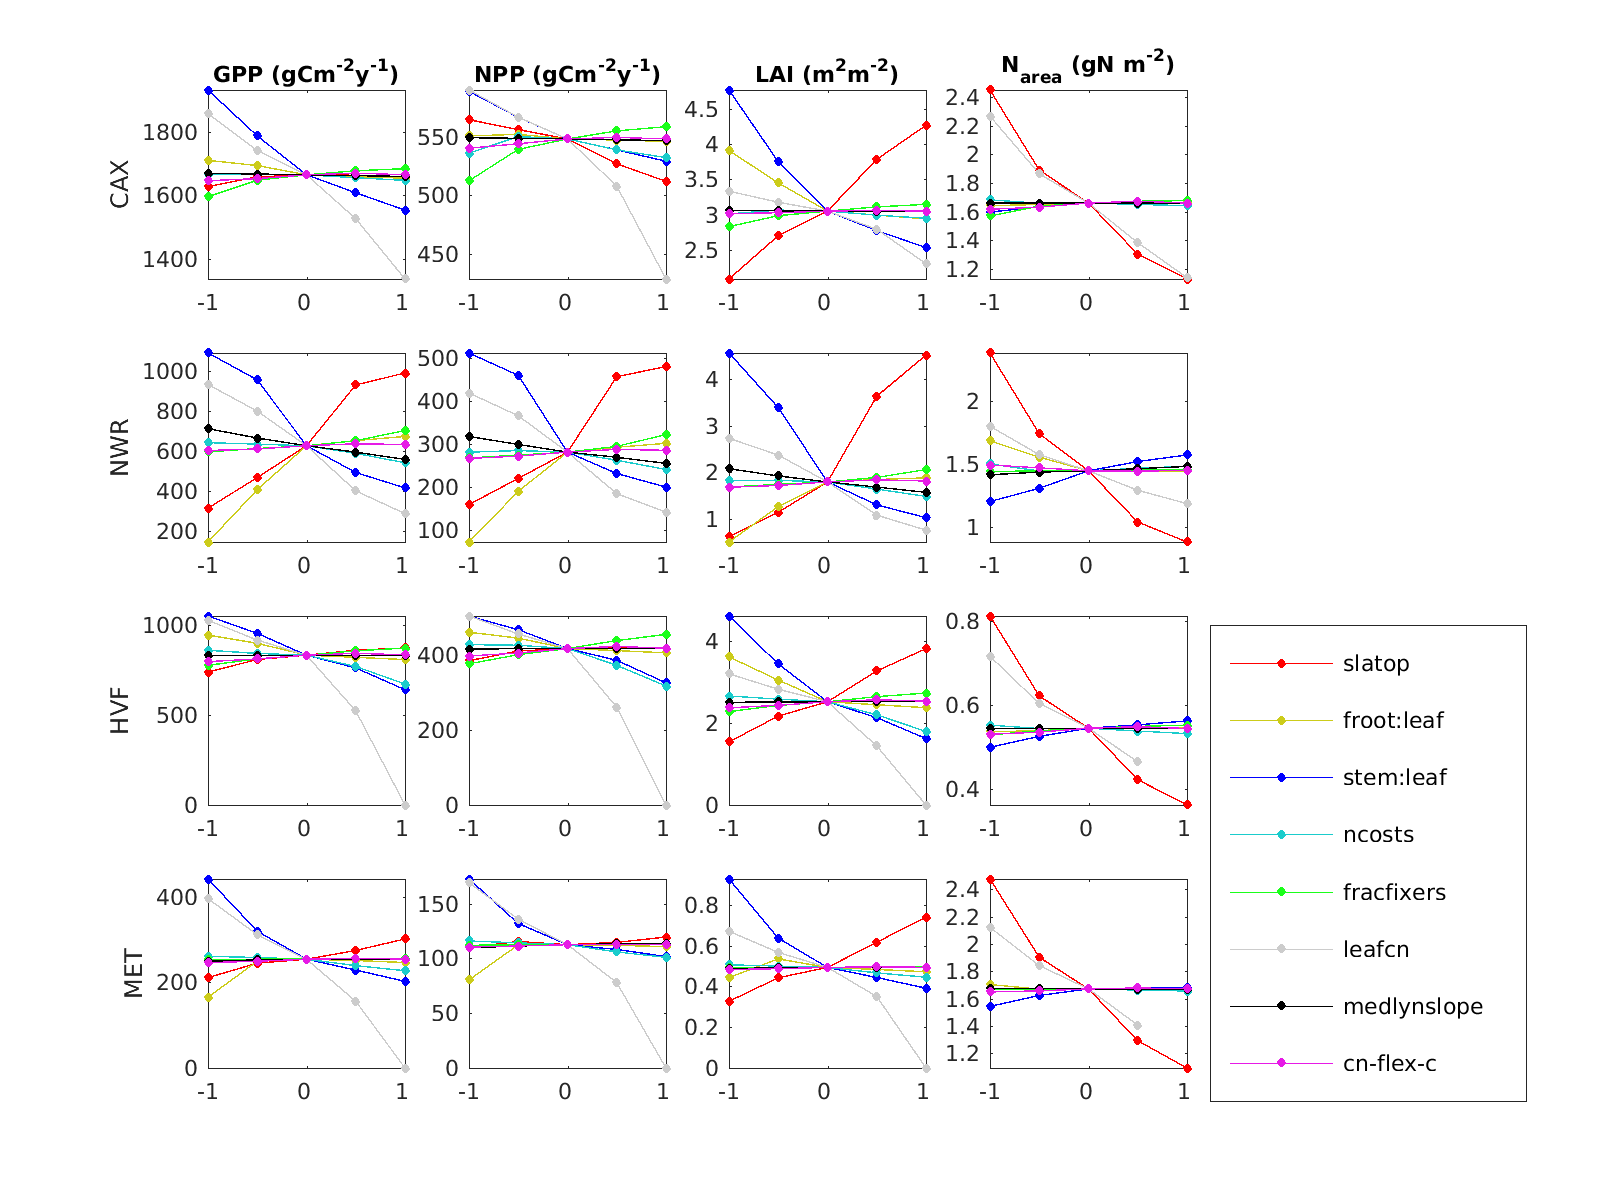
\includegraphics[width=1.2\textwidth]{matlab/figures/MAY19jp_STATE_y1999.png}
     \caption{Response of control model states and fluxes to parameter perturbation across -1 to +1 range of parameter variation (Table \ref{table_ranges}) for GPP, NPP, LAI and N$+{leaf}$ at the CAX, NWR, HVF and MET sites}
     \label{state}
 \end{figure}

  \begin{figure}[h]
     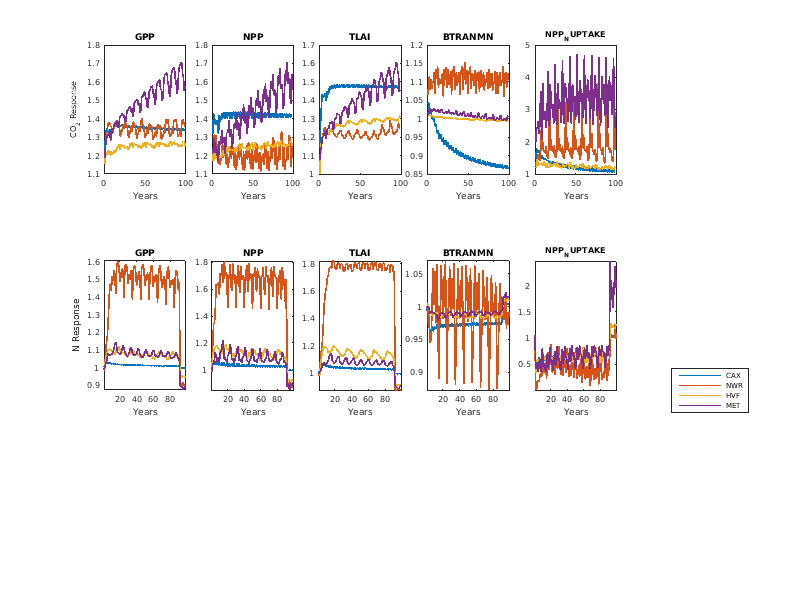
\includegraphics[width=1.2\textwidth]{matlab/figures/MAY19jp_CNtime_defpft.png}
     \caption{Fertilization responses of the default model though time since the (step-change) in CO$_{2}$ (top row) and Nitrogen deposition (bottom row) for CAX (blue), NWR (red), HVF (yellow), MET (purple).}
     \label{timescales}
 \end{figure}
     
 \begin{figure}[h]
     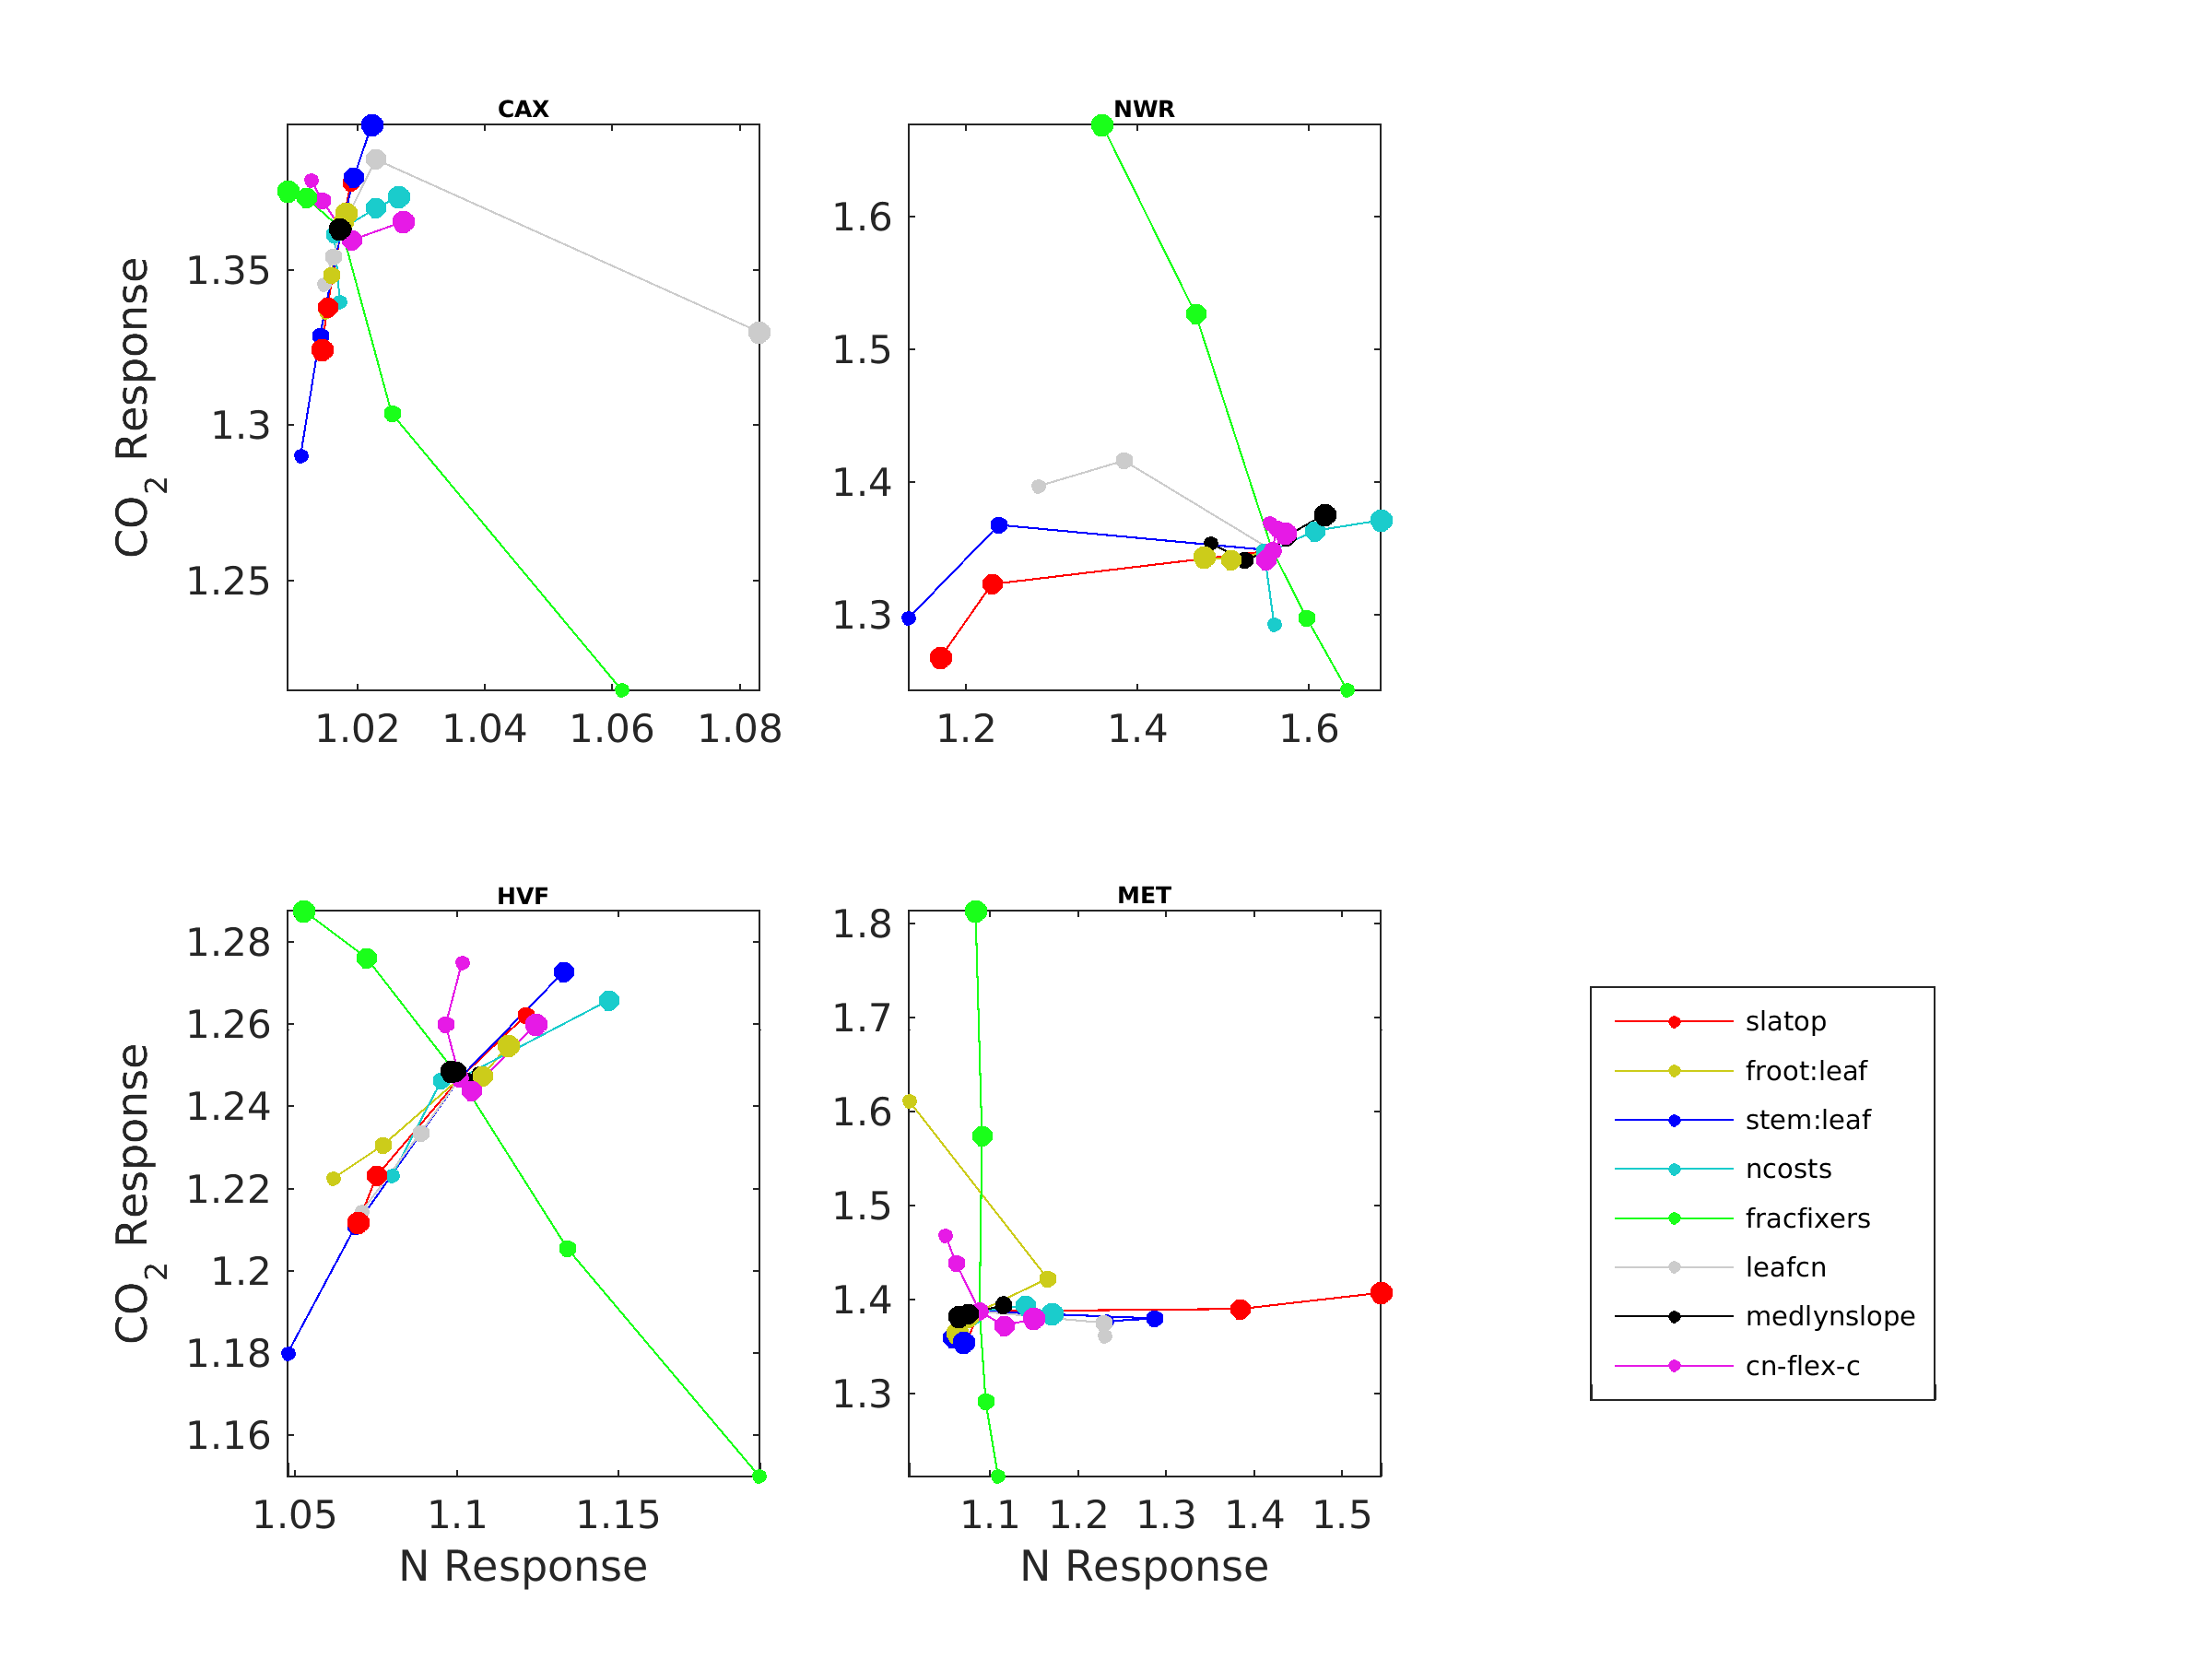
\includegraphics[width=1.35\textwidth]{matlab/figures/MAY19jp_at_relCNdep_defpft_GPP_y2013.png}
     \caption{Influence of parameteric variation on the model response (fertilized/control) to 15 years of 500ppm CO$_{2}$ and +5Kg/m$^{-2}$/y N fertilization on gross primary productivity (GPP). }
     \label{GPP_CN}
  \end{figure}

 
  \begin{figure}[h]
     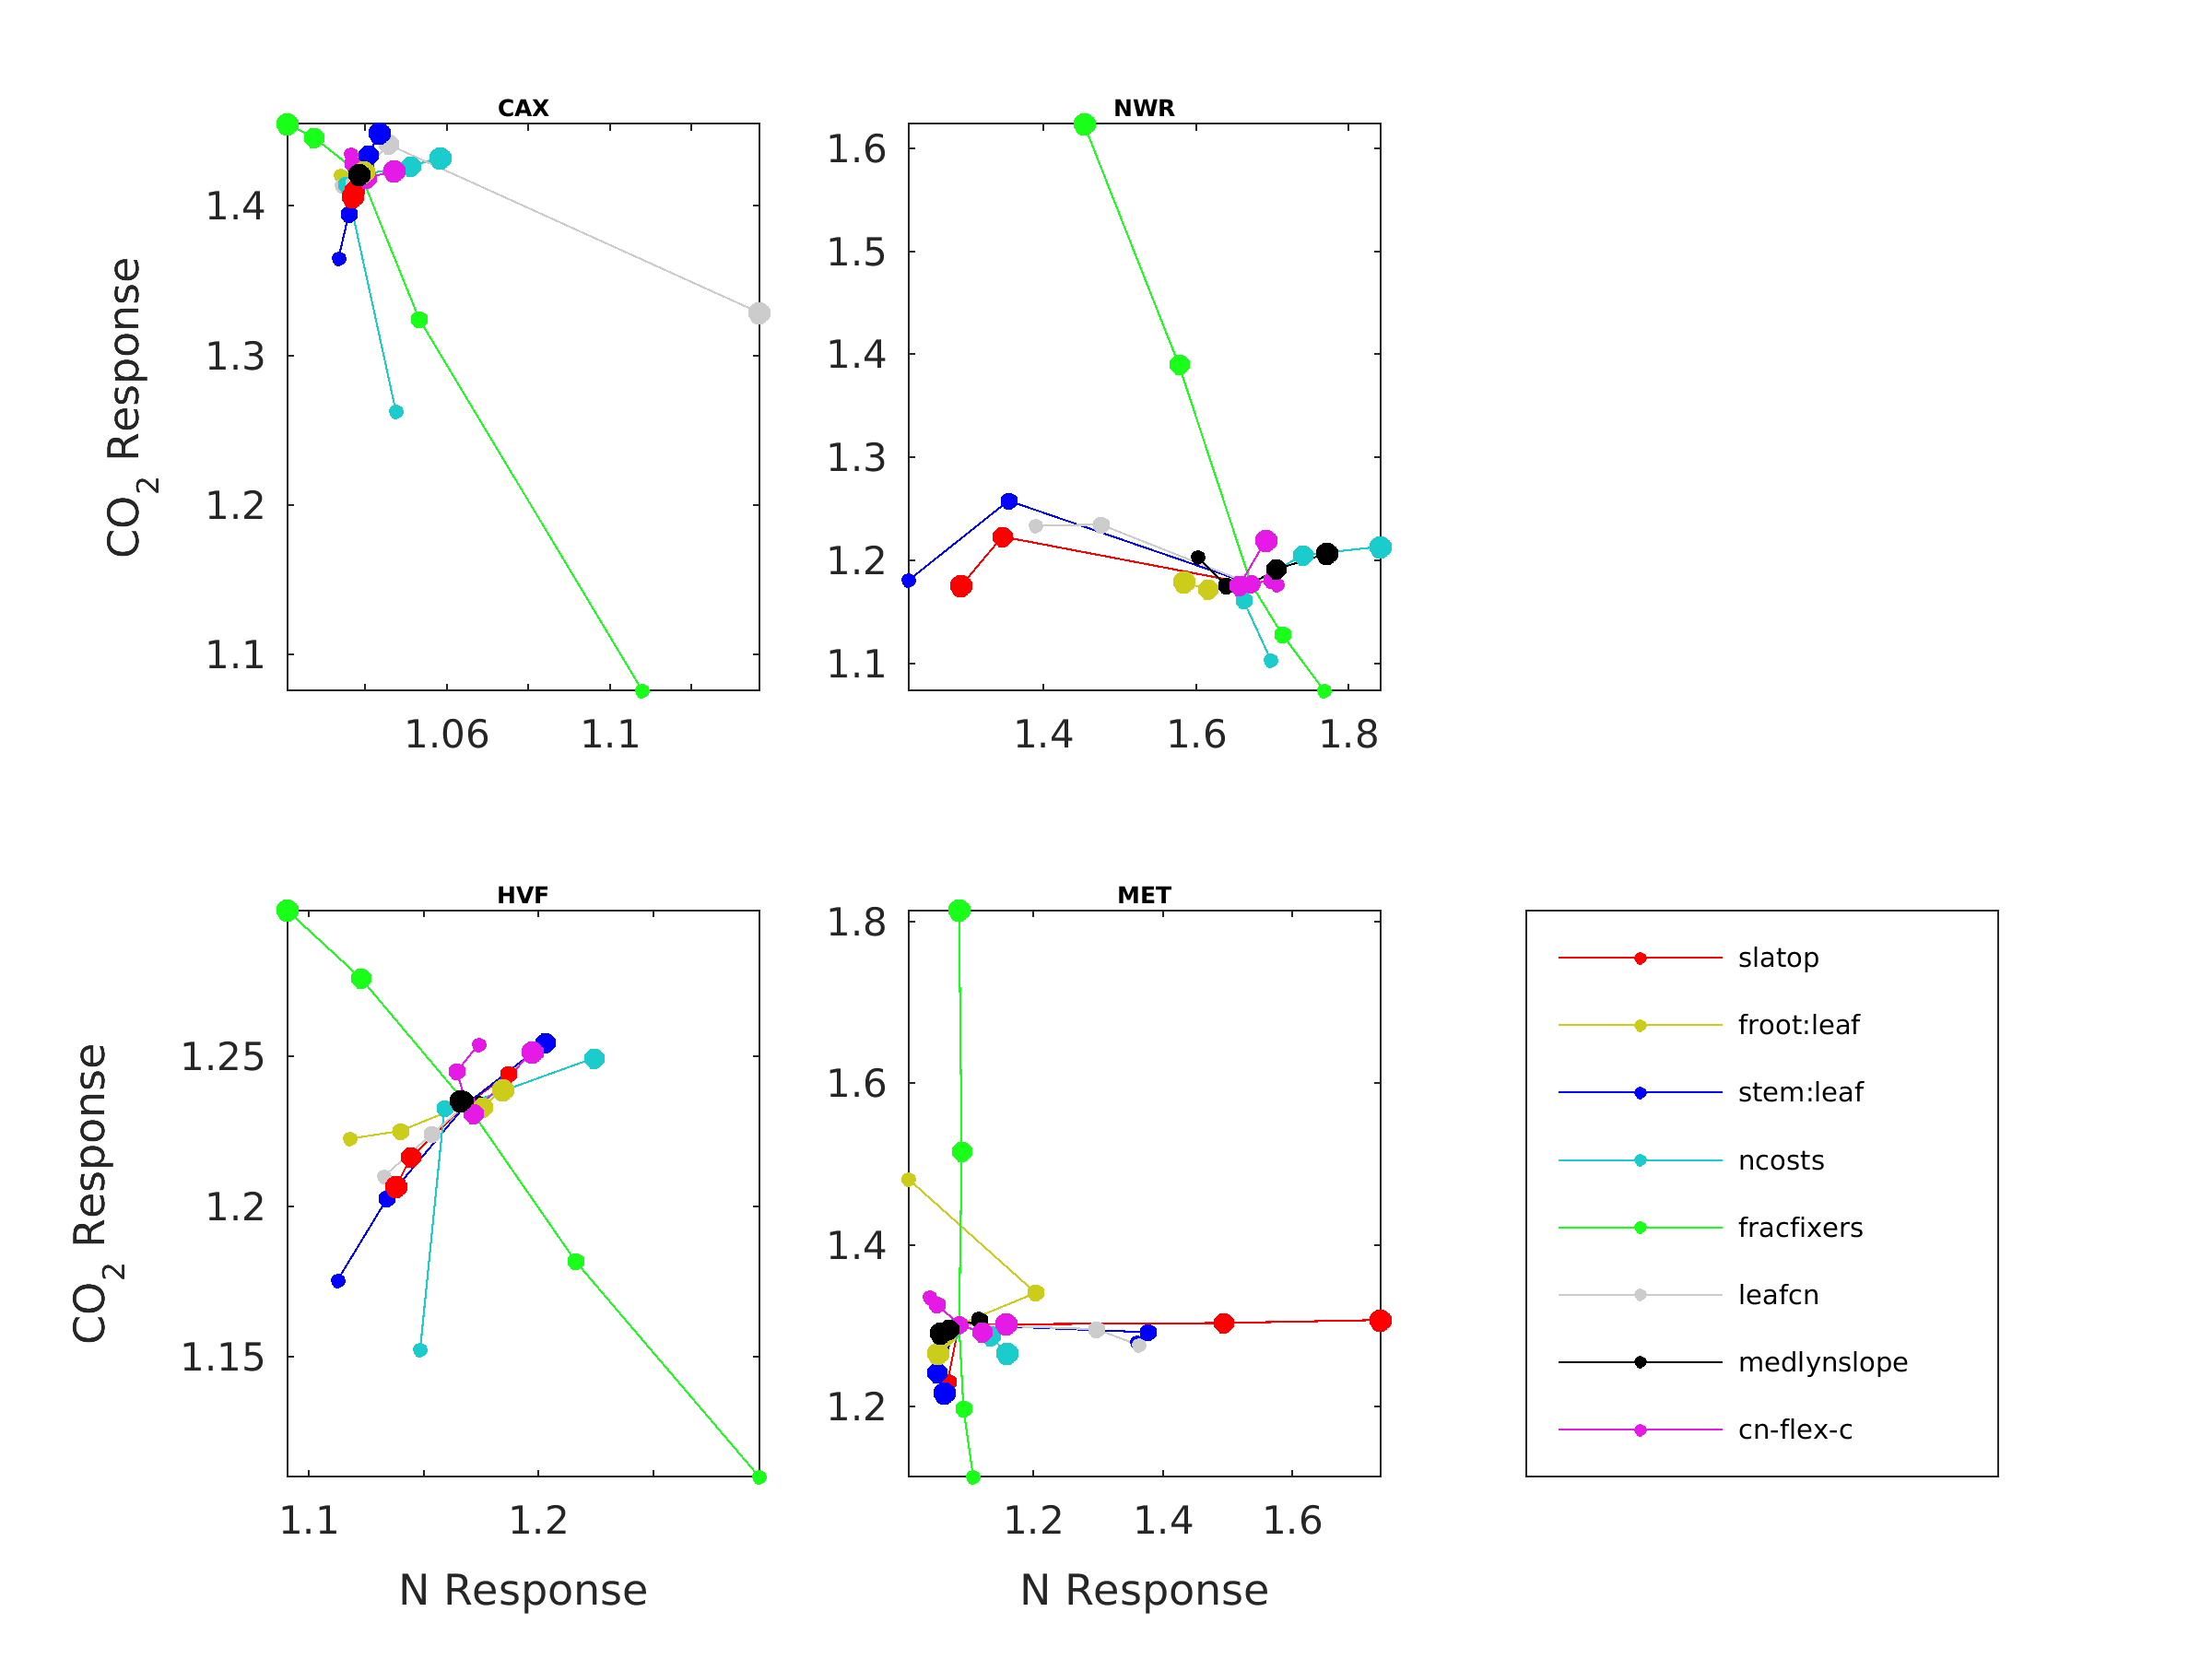
\includegraphics[width=1.35\textwidth]{matlab/figures/MAY19jp_at_relCNdep_defpft_TLAI_y2013.png}
     \caption{Influence of parametric variation on the model response (fertilized/control) to 15 years of 500ppm CO$_{2}$ and +5Kg/m$^{-2}$/y N fertilization on leaf area index (LAI). Note changes in scale between plots to show detail.}
     \label{LAI_CN}
  \end{figure}

\end{document}

